\chapter{Graveyard}

\subsection{Towards or away from} 

% Klarer gegenüberstellen
%Teil 1
When a situation requires their application, these principles are closer to \textit{responsibilities}, which one must adhere to when trying to achieve the goal of succeeding in these challenges with a group of people. It is expected of you by others or you are following a unproven principals.\footnote{
	Yes, unproven is right. Some principals have no base in testing out, but we follow them anyway.
}

%Teil 2
If the situation seems hopeless in applying them, then they may be viewed as opportunities to find a solution for the given situation, guided by those principles.

Therefore, this section is called \textit{Responsibilities and Opportunities}, capturing the dual usage.

\section{Four Responsibilities for your Team}

\subsection{Driver for a Vision}\label{responsibility__driver}

\paragraph{Set a path: Clear, consistent, constant}

A leader's primary responsibility is to find, set and drive a compelling vision that aligns with the organization's goals or sets them.\\

This vision serves as a beacon, guiding the team towards a shared future and inspiring them to work together with purpose and enthusiasm.
A clear and constant vision helps prioritise efforts and align individual contributions with the broader objectives inside and outside the team.

\paragraph{Definition of a Vision}
A vision is a future state that can be expressed as a sentence, a picture, or a goal.\\

It doesn't need to be explicitly defined in detail. Explanations can be provided if they help or are necessary in the decision-making process. However, it should be a vital part to guide action and strategy.
It is not a strategy or a plan for achieving it! In the literature, you can find distinctions between a vision and a mission statement, but the goal is to make it as simple as possible: so that it can affect decision-making today, and can be an integral part of a team or company.\footnote{
	For example, a vision can be expressed as a \textit{state} to be in, which could fall more under the category of a mission statement: \textit{Wir sind ein leistungsstarker digitaler Betrieb}. This typically indicates a mission statement rather than a vision statement. However, in this context, there is no difference.
}\\

A vision may have two parts: an internal and an external outlook. For example, \textit{Wir sind ein leistungsstarker digitaler Betrieb} and \textit{Zuverlässig $\&$ aktuell informiert: So bewegen wir München}. These two parts combined can also be a vision for a company.\\

The responsibility lies in ensuring this vision is constantly upheld and remains an integral part of the team, influencing decisions.\footnote{
	Projects, strategies, daily discussion.
}


\paragraph{Motivate Internally and Externally}
Ensuring social support, capital, and information input for the team to achieve the vision is also part of the leader's responsibility.

\paragraph{The Risk: Not having one.}
If the vision is not clear and what it takes to achieve it is not thought out—whether in terms of team capabilities or strategy—then assembling a team is risky.
The team may not move in the direction of the vision, and the selected skillset may not be complementary.

If they may do great things, does not absolve the need for a clear vision and executional strategy, it may mean, that a the team is doing great thing \textit{dispite the leadership}.

\subsection{Alignment and Decision-Making} \label{responsibility__alignment}
This involves turning plans into action, ensuring that the team is aligned and resources are optimally utilized.

\paragraph{Delegation and Accountability}
Delegation is crucial for effective execution.
Leaders must trust their team members with responsibilities while holding them accountable for outcomes.
The difference between micromanagement and effective delegation lies in giving team members the autonomy to execute tasks and finding solutions while providing support and oversight as needed, instead of evaluating the solution-finding process, and using once-own way in takeling a given problem. The focus is on evaluating the outcome of once work and how this integrated with other work and the lager vision.

\paragraph{Information Integration} The great team is the best source of information, essesion power and finding the best solutions. In the perfect setting, there individuell work is aligned with the vision. Therefore, they are able to look for alignment problems in the work of there coworkes, that either is in conflict with there owns or with the larger vision. Futhermore, there integrated understanding of the team culture allows them to function as internal feedback-giver.\\

The responsibility lies in using the team to get the best information as possible.

\paragraph{Constantly Align}
Analyzing and gather information about the outcomes of the team is the requirment, to be able to do it
This information should then be used to evaluate progress against the vision or strategy and to constantly communicate what it takes to align actions to achieve it internally and externally. 

\paragraph{Take the left decisions}
$"$Left decision$"$ refers to those crucial choices that no one want or can't make.

That different from "two-door" decisions, meaning they may have a significant impact and are not quickly reversible. If no analytical, logical, or group consensus can be reached for these decisions, leaders must take responsibility and make them. However, the goal is that the group is doing everything, to analysed and make it.


\subsection{Finding the best solutions} \label{responsibility__finding}
This requires nuces for the specific assemble of the team, the field the team is in, and 
% Team Requirement: Deeping on the vison, the field of expertise the team is in.
% Nuces: The assumtion is, that to find the best solution, a lot of comunication, testing, and adapting on new resolts.
% The risk: 
The responsibility, that 
Creating an environment that encourages finding the best solutions is a core leadership responsibility. This involves fostering open communication, promoting collaboration, and encouraging diverse perspectives.

\paragraph{Closer to the Truth: Pushing against Social Equilibrium}
For me, coming closer to the truth is assumtion, what it take for a sucessfull team. There are probably other way to set up culture, and be sucessfull. However, from that are derived responsiblities, that requires, pushing a team and once self out of a social equilibrium, by applieng heuristics, which are design, to foster quick and collective truth finding.   \textit{Note: This equilibrium, must mean, everbody is happy. It means, all action, that a social system took in a given enviroment, are heuristics, which have group cooperation, and group stability as it's funcitional goals. Again: That does not mean, that those heutristic are producing in any enviroment and at any size or time scale a stable group. Further find further explaination, ask the auther.}
\begin{center}
We sacrifice a bit comfort, for a long time success.
\end{center}

\paragraph{Memo: Coherent Decision Framework}
Clear and concise memos ensure everyone is informed and aligned, facilitating better decision-making and coordination.\\

The memo-style presentation of once work is designed, to ensure, to siffout unfinshed thoughts, which a group has to evaluated.
And allow to give persise crital feedback on for e.g. error, different solutions.
This is more work for the autor, but, it should mitegrate the risk of siffing out thoughts, which the autor itself coult done, and using the group abilities, to give target valuable feedback for once work.
As pointed out above, this is not a social heuristic for group stability, just because, this increases the risk for the author to allow a group to find something negativly associated with them. Therefore the responsiblity is, to value the risk, the author took!


\paragraph{Decision Making: Information-Flow}
The goal is not, that all information flows the person leading the group!
The goal is, to have the best decision-making progress, by using each relevant persons inside in improving or finding or stopping a presentated solution TO THE GROUP.\\

Two things are important for this
\begin{itemize}
	\item Arguments should be boucing back to as much as possible of reelvant person. This will required the responsiblity to ensure, people with reservation or general crital options, are encource to speak up, and adressing it as clear as possible.
	\item In reference to \textit{taking the left decisions}. If the leading person estimates, that a decision at the needs to made at the end, then collecting as much as independed information from the group are peramount. For this, the leading person, should talk or make his position clear only at the end. Otherwise, the information flow get's selected beforehand (social eq. heuristic). 
\end{itemize}

This collaborative approach helps surface diverse ideas and fosters innovation.

\subsection{A Great Team} \label{responsibility__great}
The responsiblity lies in that, to find, keep motivated and talented people for the group itself, that they we as a team are most able to fullfill the specifiy vision.

Also the harder responsibility lies in hown the team, that the group itself is protected, by \textit{keep away} pepole are hindering the group in fullfilling the specific vision.

The responsibly lieas, that ties out, that grouopmember goal and aspiration that is aligned with the overall mission. 

\paragraph{To be great, what does it mean?}
In relation to the overall topic of this, it means accomplishing things that are relevant for a great number of people.
Being great in this context does not necessary mean having a great number of skills, which may accomplish something. Nonetheless, having a great skillset may be an indicator of achieving great things in the future.\\

In reference to not having a clear vision and strategy, here lies the risk. People can have a variaty of skills, motivations and potential. Therefore, is paramount, to have a well thought out vision and strategy, to know, what is required to archive it. That's sounds easer then it is. It's very more often then not, clear, what is required.

To that end, the team itself should be guided in finding the best person to fit into the team.

\paragraph{Protect the vision and the Group: Keeping the promise}
% Hone your team
% Focusing attention on the overall goal: Achieving the vision for society and our colleagues themselves.
% If you have to leave, then this should not be a surprise. If the feedback cycle works, then this should be indicated beforehand.

\begin{center}
	If the promise can't or doesn't want to be kept
\end{center}

The promise is that if you join our group, then you are striving to
\begin{itemize}
	\item \textit{align your work to the overall vision},
	\item \textit{towards aligning it to the work of your coworkers},
	\item  and \textit{evaluate your own skills}, to see if they are the right fit right now to serve the team's goals.
\end{itemize}

% If it takes two years to learn specific skills, then you are more than welcome to join again.

If this promise can be kept, then the social harder responsibility\footnote{
	This process is socially hard for the team, the leading person, and the person in question, because
	nobody wants to see somebody suffer, even if it's short-term. Nobody wants to attack a fellow group member, and nobody wants to be excluded. That's what makes it very hard for everybody to go beyond thinking about this topic and actually acting on it.
} is to ensure:
\begin{itemize}
	\item The person in question has to \textbf{leave the team}, or
	\item This person \textbf{must be kept away} from the team, in order to protect the resources and focus, and commitment of the team
\end{itemize}

For evaluation, the team itself should be used for this as well. The responsibility lies in leading the team safely toward this information collection. Safe, because without practice, this is a difficult social area to be in. The upside is that everybody determines and understands what it takes to be part of the team and can reflect on themselves and may counteract before the team has to act.\\

If the leading person sees or deduces from the group behavior that a person can't or won't keep their promise, then this hypothesis should be tested by leading the group to evaluate the situation:
\begin{itemize}
	\item Is a person or are they not keeping their promise in terms of skills, feedback culture, alignment?
	\item Or is this person causing other people to drag with them?
\end{itemize}
If the group clearly states that there is some trade-off or other offset, then either the hypothesis is rejected or the leading person can state to \textit{disagree and commit} with the analysis implication until new information arises.\\

However, if the information collection indicates that the person \textit{should leave} or the team \textit{must be protected}, then the leading responsibility is to make this decision and execute it.

\paragraph{*Selecting/ Joining}
% Let Go: Recyle responsibiity: But it's going into the grave yard: Mathamtical approach, shows the weekness. Help, collabertion!
\section{Recycle Responsibilities}
\subsection{A group, but not a Team}

\paragraph{A Team} If all four responsibilities decided to be taken on for a group, then this group constitutes a team.\\

Let $ g $ be a group of individuals and $ R = \{ r_1, r_2, r_3, \ldots, r_k \}$ be a predefined set of responsibilities. If you, as the assessor, determine that all responsibilities in $ R $ are fully applied to the group $ g $, then $ g $ qualifies as a team. The currently defined number responsibilities is four. The four you find above.

\paragraph{A Group but not a Team} Various group structures and social dynamics exist. The following categories represent an incomplete set of possible groups where the predefined responsibilities $ R $ are applied to a lesser degree. In these cases, some responsibilities might not be fully met or may not apply at all.  For instance, in a collaboration group, you might assess that certain responsibilities within $ R $ are not fully applicable or not applicable at all.\\

Let $ G $ be the set of the following social groups: \textit{Collaboration, Alligence} and let $ g' \in G $ be a specific group. Let $ R' = \{ r_1, r_2, \ldots, r_4 \} \subseteq R $ be a subset of responsibilities. Various group structures exist where the responsibilities $ R'\subset R $ are applied differently or to a lesser degree.\\

Define a function $ f: G \times R \rightarrow [0, 1] $ representing the degree to which each responsibility is applied to each group, where $ f(g', r_i) = 1 $ indicates full application and $ f(g', r_i) = 0 $ indicates no application. For a group $ g' \in G $, if there exists any responsibility $ r_i \in R' $ such that $ f(g', r_i) < 1 $, or if $ R' \subset R $, then $ g' $ is not considered a team. For example, in a collaboration group $ g' $, some responsibilities in $ R $ may be applied to a lesser degree or may not apply at all.


\begin{figure}[H]
	\centering
	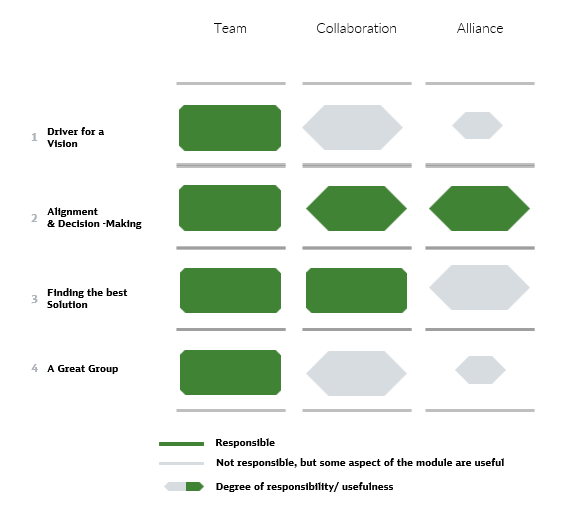
\includegraphics[scale = 0.5]{attachment/chapter_OWN/Rubric_LR_Degree_of_Responsiblity}
	\caption{Example of reduced degree of the the four Responsibility}
\end{figure}




\subsection{Collaboration: Collection of Collegs}
For the following group, the four responsiblities are seperatly evaluated. 

\paragraph{Driver for a Vision}

There are no inherent exception to set the vison!\\


If the decision is made, to lead the group either by a share assumed vision or set one for them, then restlichen responsibility are with all supparts are yours.\\




derive to \textit{set a path} with al theHowever, this social construct is more lose, therefore it is not as bounding as with a team, because a team member chosses more consicly to join a team. With college there are either not essabled by you or if essabled by you do not have as much range in protecting the vison and the rest of the group, if required, or it is different from the team.\\



\paragraph{Alignment and Decsion Making}
For that \textit{alignment} and \textit{finding the best solution} can be proviede. 

In case no path for the vision is set, then is might not be $"$your team$"$, but the concept of $"$a team$"$, which - if the responsibility is taken, can be lead a vision.

The main resonsibility lies  successing in aciving a vision.
All the same can be applied as for a team. However the social relationship differs from a team. 
On the topics of dependency, it may can have the same stronger or weaker as with your own team. 

However, the same for a team as with collaberation partner can be say, 
the are a vital part of striving together towords the vision.\\

$"$Keeping the promise$"$ might be harder to follow with the collaberation partner.

If the social bond is more like a collegtion of colleges, and no stated leading position is said, then the promise can enforced by providing the perspetive, that this collegeion of people should align there work with the other members to the benefit of all and the vision.

\paragraph{Risks: Jumping of Point}

If your vision can be reached with the collaberation or it takes to much personal ressources to achive it, in this constallation of the cooperation.\\

To have controll of the input-output selection of the group, the principal of raising this topic with the group it self and use them to evaluation the situtation of \textit{protecting the team and vision}. If the group come in there analysis to exlucde or change the structure of the group and can't make it themself, then the reconision of the group is required, that the person with the leading responsiblity is able to do it.\\
% Different nairativ, again.

As said before, if the reconition is not meet, then the option of ending the responsiblity is given.

\paragraph{Special Case: Payed Collaberation}
If the social bond is more like a temporay payed collaberation, the most important part is taking responsiblity about providing a \textbf{true expected results}. The delegation is implied and expected. Keeping the promise is not really part of if, because this needs time to get a cross. However, making the importance of the conctribution for the larger vision clear, is not a leading responsiblity, but will help a leading principal that should be applied when ever is possible.\\

In ecessence, the leading responsiblity lies mainly in \textit{delegate and accountablity}

\section{Group-isch}

There is the commonly used concept a \textit{team}. However, looking  through the lense of social groups: by accepted hirarchy\footnote{
	There are different kind of hierachies.
}, observed dynamics, individual goals and playingfield dependencies, the concept of a team get's replayied with nothing, thus get's more simplied: a working-group.

Is a team not a working-group? 

No. A team gets most commely understood as a group which get's selected by one person and this team follows the set implicite or explicite incentives or this person, based on the evluation of this provides incentives.\\


A more applicable definition is a group.
Which might be true for a lot of work-groups, it's not 
 observed, the true incenties between  the true abbility to hire or fire person, to direct orders or stire them 

\subsection{Alligence - Inspiration}
% No responsiblity in output

% Black Board: 
% D&A is still relevent to use here: Comparitive Advantage; 0



With Alligence are meant people how are believe in some aspects of the vision or can or want to use some capacity the team or collaberation has build.\\

KEEP THE Feeling of responsiblity away!!! % Regina, Isabella!!! 
%% Asses used strenght first
%% Only asess and act if they explicity ask! More like cusotmers!

The first two group categories define groups, which are part of the effort to archive the vision and it's strategieg goals. The category \textit{alligence} require no leading responsiblity as discribte here. In that case, it's more like inspriation to that kind of group. But, there is no responsiblity in there output! That is cruial. This category should help to distingish, between feeling responsible, to everyone.
% Walter, Regina, other department


\subsection{Leadership}
- Making decision, but not "A great team".
Es soll nicht vollständig sein.
Das Ziel soll sein, dass es koheränt und verständlich ist.

\paragraph{Totally loos}

Finger Pointen Everbody to Everbody
Pointing to the purpose 
People: Problem: Left behind (Group has to evaluated: Not I. I have to Forster it, if I see it. And I have to make the decision, because it’s painful 

Identify: If skills, feedback, or purpose can‘t be reached with them.
I want that we, are prode, in achieving it. SamtimeS hard 
————-

Noch erweiterbar:
———



The tool of choice would be a strategy to point the way.\\

A vision is just a future state. Normally, there is no path shown that ensures a team today can move towards this vision state in the future. 

A strategy would not only be a path from today to the vision itself, it would also be relisation, how this vision would look like. Sort of in the same way, as objects and key results interact with each other. A object is just a goal. The key results are mostly definied not derived indicator of this objective. In similar means, definies a strategy $"$a$"$ expression of the vision.

----
Even so, some of the vision statements can mostly not be 

To align futher desicio

% There is only now! And ever will be!

% Likeleyhood: To estimate, what comes next. Prediction the next words. The problem is, that if you are not testing your feeling, if you thought, that you could predict, what comes next

% A Vision is a theortical model of the world!
% This model, does not exist (Invetion or Discovery of mathematics). It even does not exist on pages.
% The goal is, to make prediction about the world.

The goal is, that other people re

Organsiting Schema: Aling ressource

A strategy may be the first realization of the vision.


For example, YouTube's mission statement is \textit{to give everyone a voice and show them the world} and Alphabet \textbf{4Es: Earn, Entice, Expand, Experiment} is it's current stategy. However, there is no single strategig realization of this vision. It is the first  
...
Instead, various strategies must be implemented and adapted to work towards achieving it.

As circumstances change, leaders must continuously reassess and update the strategy to ensure it remains coherent and aligned with the set vision. Regularly updating the strategy is essential to keep the team focused and adaptive in a dynamic environment. However, this does not mean that the vision has to change. It indicates that the path or expression of the vision may need to be adjusted.

\paragraph{Knowing the difference: Vision Max or Team Max}
There is a difference, between maximizing vision or maximising the input.

What is meant by that is, maximizing the vision is, constantly finding and keeping the best team member and ressources to strive to the vision. The focus is to doing everything to position the team or fulliel the vision, and not lowering any standards. On the other hand, \textit{maxizing the input} with thegiven ressource and teammember cabailities the best relesation of the vision will be strived at.

The responsiblity lies in that, know the own capacity to understand, what principial can be applied. The assumeion is, that follow the one or other prinzipal is not a consiuse choose, but rather a behavior for ever endover. However, I knowing the capacity or whishing to change it, is important for setting the vision or subgoals and in communicating this to the team and letting new person know, what to expect.

For example: If maximizing a personal teammembers potential is not suffient to achive ,


There is a different responsiblity: Honouring the commitment, other teammember made to the vision including the archivment of the strategiy great things.

\paragraph{Finding great Teammates for great Teammates}

% The goal is not, that they learn from me, that they learn from the great team mates!


% Refactoring II

%% Tools
%%%Vision (Output) Maximizing

%%%Team (Input) Maximizing

Until now, I did this. With the given input, to reach a certain goal. However, if the input was not sufficient, then the goal was adjusted.

Bei größeren Zielsetzungen und größeren Verantwortung, birgt die die Input Maximizierung Probleme.

... Probleme
Colleges Bases: The risik is, that it can be demortiliseing, pull und pushing other people. Not everybody has the patents for it.

More work has to pick up by other team mates

And you as a leader don't hourner the commitment each teammember made to the vision, by allowing team dynamcis or not sufficent teammembers dafür sorgen, dass die Zielbereitschaft andere Teammitglieder nicht erreicht wird.


... Meine Führungsverantwortung:
Mein Versprech

Personen geben sich der Vision und Erreichugn hin (für diese Personen habe ich ebenso verantwortung); Wenn Mehrlast auf Personen fällt, welche Teile des Team zu langsame für die gegeben Herausforderungen sind, liegt hier ebenso die Verantwortung bei mir.


Bei größeren Strategien Zielsetzungen, liegt jetzt hier die Priorität (Lernen, die zu tun.)
Mehr auf Vision Maximizerung.

Die besten für die besten finden!


% Refactoring I
Der Schwere Teil: Entscheidungen für das Team, die Vision und Kunden treffen. Kein eigener Standard setzen.
- Entscheidung in den ersten Wochen: 
- Kontinuierlich: Commitment der Teammitglieder wertschätzen, wenn der Einsatz von ihnen dadurch geschältert ist, oder sie auch nicht die Vision erreichen.
- Neue Strategie, welche der Vision näher kommt;Neue Capacitäten werden benötigt. Selbst durch Loyalität muss dann ein transit gefunden werden.
- Low Performance Part vs Priorsierung von Ressourcen; Es ist nicht nötig, nur low Performance zu entlassen.

Bisher war es so, dass ich mit dem geradbeit habe, was da war und gegebenfalls meine Vison/ Strategie angepasst habe (nach unten korrigiert).
Jetzt bin ich verantwortlich für das Team, dass die Vsion erreicht wird, und den Input wähle ich aus und pflege ihn.

Deletegat, accountability, quality: Integrate Team results (Zu einander bounces); 
What does it mean, to mean great. Is very abitray.


Continuosly keep it great

The aspekt is to make Continuuesly Assembe a great team for the vision.

—-

%%%% Refactoring





Finding talentent people, who will de

maybe given a more true statement.
——
What I do, is using the talent a got in the best possible way. 
There is a way, if the vision requires cabbilities, which are not here anymore.

Make a cut, as quick as possible!
Loyatcly. 

There is a difference between the zielzustand.

Making a quick decision - Couple weeks, less then a month.

There are here for me, I‘m there for them.

If the vision evolves or the required stategy cabaility are increasing, then a discussion needs to be.


The loc

First, we are here for other to archive the vision. By doing it we bond over it, by creating something great.

What to do, if cabilities are not sufficient after a certain time. 
The vision and the goal dictates.
Responsibility to make decisions 
Horner the commitment of the team, of there commitment to the vision and enshojsdofias.
for the team, there commitment to the vision and 

Maybe category of quality.
There is then a lower cabinet part of the team as well. 
this ranking, determine the priority and resource investment.

Make the investment Gebern, bewusst, wo die Priorität liegt.
Ebenso, kann auch die Entscheidung getroffen werden, nicht jemand weiter zu führen im Team, weil die Ressourcen für andere Themen oder Personen aufgewandt werden müssen, im Bezug für Visoin.

Meine Persönlichkeit erlaubt mir nicht, anhand eines persönlichen Standard, Selectionsentscheidungen zu treffen.
Die 

Eine eigenen Einschätzung ist das hier.
Diese Einschätzung kann dann bewertet werden.
Sicherlich, nicht alle Punkt, die anderen einfallen werden hier aufgefasst. 
Was hier aufgefasst ist, sind die Punkte, welch für mich ein bewussteren Anspruch erfordern. Dinge, welche hier nicht erwähnt sind, wo automatische Verhaltsweise ausreichen oder automatisch kommuniziert werden.


\paragraph{Lose* Personal Guide Finding Value}


So, the topic is called: Finding Value!
Inset of finding the opertunities with the greates marginal value for satificfation. (This can by strategy power, but it can also be just temparary satification. Then again, an other operturnity can arrise, which has a high margina emotional value)

Two guiding this:
- Find value, where the margial satification rate is very high. 
- Then Delegat  Accountablity, lead team to develop X to give person or a group the strategy power.
Note: This is different, from a system, which very body just have to fill in and "bedinen". For example. Urlaubsplanung: This is a system (Exeption can be made), that has no stratgy power for somebody. Therefore no satifaction feeling. Then the accosition is, that I provided this statgy power for them.

I'm not also relevant for quick relevae.

Strategy Power, to allow other to have strategy power


-----

Deeping on how 

If a vision has a whidely accepted goal\footnote{
	This means, it's understood, can be whidley evaluated in the same way, and or can 
}

Strategy thinking: If a goal, project or other effort is set. Then it is vital, to think about, what team member and 

and it thought out, what is required to achive it. Then there are two approaches, to achive them.

The best are determined, by the group itself.
Most of the time, 

Strategy Positioning: With the best people*

% Check, if a principal or concept is actually integrated, before expanding it.

\paragraph{Internal Mechanism: Don't let yourself confused by language.}

A good $"$internal mechanicsm$"$, which feels like a thought, might not always find an equality good verbal and mathematical description!
% Evaluate mechanism: For you self
% Close learning: By observation
% Transferring it into the world of language*mathematics.
% The problem might accure, by translating it into the world of language, the mechnism gets broken, mistranslate or has a feedbackloop, and reshaping the orignal internal mechnaism.
%See, NFM. Furhter definition is not always necessary. It might even be  hinderring.

% For me, a mostly simple word-accoziation helps me, accaction this internal mechnaism, which then allows me, to evaluate a given siuation and make a decision. That makes it problematic.

\paragraph{Knowing the difference}
If we have this, we can only acvhice this.
If we have this goal, when need this.
% Philopsy stand or External Need or Pressor.
% Hourner Commitment by other team members, if thery are commited themself to on or the other.
% It is also possible, that it is interly self servering. If nobody want it or it is unclear, how the archived goal, is integrated into the live of others, then pursure of the goal, is not 
% Communicate: That I have a certain standard. And I'm not letting go of this. If you are not
% Communite of One/ Community of Multiple: 
% I see, I can not make it work, that it is something interlly free form my.
% Communicate: Culture of Excellence vs. Input maximizing. It's a strategy capacity, to position your self as best as possible, to achvie our goals.

\begin{comment}
	% Delegate and Accountablity
	% Reflextion of the day: 
	% From the perspective from yesterday
	Leadership: Finding the right component for the team.
	Derived from willingness to Keep the promisses
	% 
\end{comment}
\paragraph{What to promote}
Finding the right balance between providing freedom and learning from the best is crucial. Leaders should create an environment where team members have the autonomy to explore and innovate while also learning from experienced mentors and established best practices. 




\paragraph{Commitment to Leading the Team}

The responsibility I see is to find people who have indicated or already proven that they are capable of achieving great things. This is relevant for the team itself, to have team members from whom to learn, strive, and be pushed by.


\paragraph{Push, to make more possible}
Leaders should constantly push the boundaries of what is possible. This involves challenging the status quo, encouraging the team to stretch their limits, and fostering a culture of ambition and perseverance. By pushing for more, leaders drive continuous improvement and inspire their teams to achieve greater heights.

\paragraph{Lasy, abmbious people}
To to avoid them.
Speciall, they get mad

\subsection{Objectives}

		% Navigation Us to Solve Great Things ::: NU-SGT
		% Is not leadership to keep a social group togehter
		% Is not leadership in having recource and permission to decision over.
		% Is about finding a way with other to solve great things.
		% I don't like navigating. More 
		% Prinicpals for achieving great things together 
		% My thoughts (CDF), how to find the best solution togehter.
		% we can collectivly solve great things
		% First principals! Social Dependecy, like contract obligations, ressource allocation. 
		% Navigation Us to Solve Great Things ::: NU-SGT
		% It's not leading in a sence that there is a reporting structure.

%If I want to achieve something, where I need a group of people (a team, collaberation, alligence), what responsiblity do I see or set axiomatics, in oder to achive the best solution.  

%Contiunuously, working togehter to achive something great. Prolong-Time

% #PT-WGT : = For a prolong Time working on something great togehter!

Thining about what I would use as guidelines for 
- mechnisam (Best solution), principals, responsiblities (todos: alignment, vision).

in order to strive togehter towards something great (worthwhile/ challenging).


WTC-PT := Working togehter on something Challenging - for a prolong time.  

How I think is the best solution for challenges together as a team. You are the person who are wanting to take on those challenges.

How I think the best solution is for initial template for achieving challenges to get short if you are the person who wants to achieve those challenges and what you partial role in it is 



WTC-PR := Principles, Responsibilities and Mechanism - for working together on something challenging, over a long period of time.



\begin{center}
	Lookout for worthy Opportunities! Don't take everything.
\end{center}
To full fill the vision, more people the your team are required.
% Part of my vision for the SBM, is to have a gras-rout digitalisation effort form the bottom up as well as big project from the top down.
% For this: I need a great team, to build the infrastructure, that departments, can use them, and enable them.
% Enable it-affice, nerdy and percise people to part of the digitaliszation effectors.
% Okay: But what I do now, it's great. I think about, if this is usefull, and if I really, can use it.
% But think about this more long termin. I think about "Delegate & Accountablity" for other people as well. 
% Where Do I want to end up.
% My approach is, to cut them out. Please: Protect you team. Bad collaberation.
% Do I have to put it con the graveyard?
% Problem, I want I team, therefore
% Difference between Delegate & Accountably & Alliance, and Coperation
% Culture of collaaberation: 
% There is not always, in my case "a team" which can be represented on an org-chart.
% There are people and topics, I feel responsible, to lead them to this vision: This can be "a Team" or collaberations.
% Then there are people, that are alliance, which may want to particapate in my vision vision or I build one for them, but, I do not feel responsible to lead them to success, because, the don't or can't keep the promis!
% People, who want to work with me! May evolve into a team like carater. 
% That's a better 
% It's not about th
% People, I feel responsible for, it the endproduct, of achiving the goal.
% Then there are topics, which
% Be there by osmoses:
% It's not about a team. Degree of connection: Be a part of / allignet.
% I think about, if there is some sort of degree of closencc.
% Core principals. 
% X / Collaberates / Alligence
% The feeling for a team, which you are responsible for as well. 
% Leading, without a team ()

To feel responsible for everything is as difficult, as to feel responsible for nothing or the wrong things\footnote{
	Very losely that means, wrong are the topics, which indicate, that are very likely have no impact on set goals.
}


To that end, the destinaction may be made between
\begin{itemize}
	\item your team,
	\item alliance,
	\item inspiration*
\end{itemize}

The degree of resonsiblity.
% I need some sort of acor.
% What is it, what I really want, I want. Don't build the architecture.
% Not everbody belongs to you team who is great. 
% Not everbody.
% Feeling responsible is a scare ressources.The idear is, that 

For all the people of you great team, the respo
All the people that in the team, need to be great.

 team, a cooperations for the mission or adjasend example.

There is a difference between your 
\begin{itemize}
	\item a team
	\item alience % Cut aligende, or don't take them, if there are not worthy anymore; Optional: Feel responsible for there goal is well; Definitly, see, if there are 
	\item inspiration: mindset, output, and protection: Be there for them!
	\item cooperation: nur output; Not mindset
	\item aligence: Shareing core visions aspects. But the output of there work is not part of a leading responsiblity.
	 Not responsible for there output:
\end{itemize}
MayBe I should write it out: I'm still excite, to expand this.

Beside your team!

% Team
% Colleges
% Leading by but no respoinsiblit

3.4 Lookout for worthy Leading-Options! Don’t Take everything.

Unterschied, 
Direkter Führung! 
MEIN Team 
ODER Meine Verantwortung (Kooperation)
UND Begleitende Führung von anderen (Nicht verantwortlich für ihren Output: Ich helfe, ihnen, IHRE Ziele zu erreichen!!) Sie gehören nicht, zu meinem Team Am Bsp. von R. Sie gehört NICHT zu meinem Team. Würde sie dazugehören, würde ich sie das Team verlassen müssen.
Aber Achtung, mache mal ist es gut, Optionen auszusparen, um Zeit und Rerscourcen für andern zu nutzen, selbst wenn diese noch nicht da sind:

A vision may have two parts: an internal and an external outlook. For example, \textit{Wir sind ein leistungsstarker digitaler Betrieb} and \textit{Zuverlässig $\&$ aktuell informiert: So bewegen wir München}. These two parts combined can also be a vision for a company.\\
